\documentclass[12pt]{article}

\usepackage{amsmath}
\usepackage{amssymb}
\usepackage{enumerate}
\usepackage{enumitem}
\usepackage{booktabs}
\usepackage{csquotes}
\usepackage[margin=2cm]{geometry}
\usepackage{hyperref}
\usepackage{tabularx}
\usepackage{tikz}
\usepackage{listings}
\usetikzlibrary{patterns, shapes.geometric, positioning, bayesnet, backgrounds}

\usepackage{titling}
\setlength{\droptitle}{-7em}
\usepackage{titlesec}
\titlespacing\section{0pt}{12pt plus 4pt minus 2pt}{4pt plus 2pt minus 2pt}

\usepackage{color} % Optional: for custom colors

\definecolor{codegreen}{rgb}{0,0.6,0}
\definecolor{codegray}{rgb}{0.5,0.5,0.5}
\definecolor{codepurple}{rgb}{0.58,0,0.82}
\definecolor{backcolour}{rgb}{0.95,0.95,0.92}

\lstdefinestyle{mystyle}{
    backgroundcolor=\color{backcolour},   
    commentstyle=\color{codegreen},
    keywordstyle=\color{magenta},
    numberstyle=\tiny\color{codegray},
    stringstyle=\color{codepurple},
    basicstyle=\footnotesize,
    breakatwhitespace=false,         
    breaklines=true,                 
    captionpos=b,                    
    keepspaces=true,                 
    numbers=left,                    
    numbersep=5pt,                  
    showspaces=false,                
    showstringspaces=false,
    showtabs=false,                  
    tabsize=2
}

\lstset{style=mystyle}


\title{Project Update: Job Training}
\author{Jacob John, Sai Ganesh Nellore, Michael Hartmann, Shravan Srinivasan}

\begin{document}

\maketitle

\section{Big changes}

We've changed our project entirely from the impact of exercise on depression to the effects of job training on employment and revenue. When working through depression datasets, we realized that we either didn't have enough data or confounders. The Dehejia-Wahba subset (1999) \cite{dehejia1999} of the LaLonde dataset (1986) \cite{lalonde1986} was an excellent choice for this course as it comprised an observational and an experimental dataset with all its confounders and no missing values.

\section{Causal graph} \label{sec:graph}


\begin{tikzpicture}[>=stealth, node distance=2.5cm]
    \tikzstyle{format} = [draw, thick, circle, minimum size=1.5cm, inner sep=1pt, fill=white, text=black]
    \tikzset{every path/.style = {draw, ->, very thick}}

    % Top row
    \node[format] (age) {age};
    \node[format, right of=age] (black) {black};
    \node[format, right of=black] (hispanic) {hispanic};

    % Middle row
    \node[format, below of=age] (marriage) {marriage};
    \node[format, right of=marriage] (education) {education};
    \node[format, right of=education] (re74) {re74};
    \node[format, right of=re74] (re75) {re75};

    % Bottom row
    \node[format, below of=re74] (treat) {treat};
    \node[format, right of=treat] (re78) {re78};

    % Edges (placed before nodes to ensure they are in the background)
    \begin{scope}[on background layer]
        \path[->, very thick, red] 
            (age) edge (marriage)
            (age) edge (education)
            (age) edge[bend right] (re74)
            (age) edge[bend right] (re75)
            (age) edge[bend right=50] (re78)
            (education) edge (marriage)
            (education) edge (re74)
            (education) edge (re75)
            (education) edge[bend left=40] (re78)
            (marriage) edge (treat)
            (marriage) edge (re74)
            (marriage) edge (re75)
            (marriage) edge[bend left] (re78)
            (hispanic) edge (marriage)
            (hispanic) edge (education)
            (hispanic) edge[bend left] (re74)
            (hispanic) edge[bend left] (re75)
            (hispanic) edge[bend left=70] (re78)
            (black) edge (marriage)
            (black) edge (education)
            (black) edge[bend right] (re74)
            (black) edge[bend right] (re75)
            (black) edge[bend right=60] (re78)
            (re74) edge (re78)
            (re74) edge (treat)
            (re75) edge (re78)
            (re75) edge (treat)
            (treat) edge (re78);
    \end{scope}
\end{tikzpicture}

\begin{itemize}[itemsep=-0.25em]
    \item \textbf{treat}: 1 indicidates job training was provided, 0 indicates that the individual had to fend for themselves.
    \item \textbf{age}: Report age of the individual at the beginning of the study.
    \item \textbf{educ}: Total years of formal education.
    \item \textbf{black}: Binary indicator (1 = individual is Black, 0 = otherwise).
    \item \textbf{hispanic}: Binary indicator (1 = individual is Hispanic, 0 = otherwise).
    \item \textbf{married}: Binary indicator (1 = individual is married, 0 = otherwise).
    \item \textbf{re74}: Real earnings of the individual in 1974, before the treatment. This allows for a more extended view of their economic status.
    \item \textbf{re75}: Real earnings of the individual in 1975, before the treatment.
    \item \textbf{re78}: Real earnings of the individual in 1978, after the treatment.
\end{itemize}

Note that all earnings are adjusted for 1982 US dollars thereby circumventing the need to adjust for inflation.

\section{Counterfactual function} \label{sec:counterfactual}

Assume $Y$ represents our outcome variable, i.e., {\tt re78}. Our set of confounders is $Z=$ \{{\tt education, re74, re75, black, hispanic, married}\}. $A$ is our intervention variable which represents {\tt treat} or job training. Our derivation for the counterfactual function looks below:

\begin{align}
P(Y^a) 
       &= \sum_Z P(Y^a \mid A=a, Z) P(A=a, Z) \tag{1} \\
       &= \sum_Z P(Y^a \mid A=a, Z) P(A=a \mid Z) P(Z) \tag{2} \\
       &= \sum_Z P(Y \mid A=a, Z) P(A=a \mid Z) P(Z) \tag{3} \\
       &= \sum_Z \underbrace{P(Y \mid A=a, Z)}_{Y \sim A + Z} \underbrace{P(A=a \mid Z)}_{\text{propensity}} P(Z) \tag{4}
\end{align}

\begin{enumerate}[itemsep=-0.25em,label={\arabic*.}]
\item Marginalizing over $Z$.
\item Chain rule: $P(A=a, Z) = P(A=a \mid Z) P(Z)$
\item Consistency: $P(Y^a \mid A=a, Z) = P(Y \mid A=a, Z)$
\item Assume: $P(Z) = \frac{1}{N}$
\end{enumerate}


\subsection{Assumptions}

In our causal graph, we can't d-separate our outcome from our treatment by conditioning on our confounders. One way to see this is by seeing that {\tt education} is a collider. When unobserved, it blocks the path from {\tt age, black}, however, it unblocks the path from the outcome to the treatment. Now, if we condition on it, it opens up a path. This is why we can't use the backdoor criteria. We can't apply frontdoor as we have no mediators.

For our derivation, we assumed conditional consistency in Step 3. We can't use conditional exchangeability as we're assuming confounders such as {\tt age}, {\tt black} and {\tt hispanic} to have a dependency on {\tt re74}, the outcome and the treatment (and so forth).

\section{Estimation and Interpretation} \label{sec:estimation}

Due to our complicated confounding, {\tt DoWhy} fails to find any estimators for a backdoor estimate. However, there are two ways we are going to calculate this estimate:

\begin{itemize}[itemsep=-0.25em]
\item{Based on our point estimand above, we can regress over our treatment and confounders to calculate an estimate of our Y. We then calculate propensity using our confounders.}
\item{In the original paper, they created matched stratum based on propensity and took an average causal risk difference of each strata. This is what we're currently using for our causal estimates, we're iterating through a list of number of stratas and choosing an appropriate number based on our observable estimate.}
\end{itemize}

For propensity, one way is to regress the treatment on the confounders. An alternative approach is to use k-means or other clustering methods for matching and then comparing within stratas. Our forthcoming goal is to create stratas that are interpretable so one can say that the effect is more apparent for a certain race, pre-treatment revenue, etc. Furthermore, we also found a list of methods to try via Sizemore's Blogpost \cite{humboldt_matching}. Some of these cover Nearest-Neighbor Propensity Score Matching using propensity scores calculated through logistic regression, random forest, and XGBoost.

\subsection{Point estimate}

Albeit, the same, there are multiple ways to calculate our point estimate or outcome. We are planning to look at the following:
\begin{itemize}[itemsep=-0.25em]
\item{$E[re78^{treat=1}] - E[re78^{treat=0}]$: This is the counterfactual treatment effect for the post-treatment revenue{\tt re78}. This is the standard approach followed by Dehejia and LaLonde.}
\item{$E[\frac{re78}{1000}^{treat=1}] - E[\frac{re78}{1000}^{treat=0}]$: Inspired by \cite{english2016causal},this is the same difference as above, except we divide revenues and represent them in the 1000s. This way models like linear regression should be able to converge faster.}
\item{$E[(re78 - re74)^{treat=1}] - E[(re78 - re74)^{treat=0}]$: This is the counterfactual treatment effect for the difference in revenue pre and post-treatment. This tells us how much someone's revenue increase due to the treatment since participants tend to have different revenue pre-treatment and we need to account for it.}
\item{$E[employ^{treat=1}] - E[employ^{treat=0}]$: This represents the difference between the rate of employment between the treatment groups. Rather than looking at revenue, we assume anyone with a salary is considered employed and see the proportions before and after treatment.}
\end{itemize}

\subsection{Interpretation}

Our causal risk estimate would allow policy makers to understand the scope of job training for the disadvantaged. The original paper described this cohort as ``ex-drug addicts, ex-criminal offenders, and high school dropouts". Since we're working with a male-only subset of this data, we're limiting the applicability of our subset to the male disadvantaged population of the late 70s.

The organization behind the program estimated a cost of \$6,800-\$9,100 per participant for training. An interesting way to think about the benefit of job training would be to see whether the expected increment in annual salary would justify the investment in the program. Albeit, the salary increment for those with higher pre-treatment salaries would be diminishing.

Our employment based estimate, although simple, can guide policy makers to understand the impact of job training on jail recidivism. An extension of this study could be used to help understand how job training could help employment and hence reduce jail recidivism (employment would then be a mediator). A similar study can also be found by Rodolfa et al. \cite{rodolfa2020case}

\section{Synthetic data} \label{sec:synthetic}

We use the observational dataset to obtain an estimate of the population statistics and use this to sample a random ethnicity (black, hispanic or white). We sample ``treat" with $p=0.25$ and increase $p$ by $0.25$ if ``nodegree" is 1 and (independently) by 0.25 for if the person has no degree.

We also assume that impact of education is limited to to ``nodegree" (encoded by ``at least 12 years of education" in the dataset) rather than the number of years spent in school. Because the people under consideration are already out of school, we assume for simplicity that this variable does not depend on age (i.e. people never go back to school), but only on ethnicity and sample with the corresponding conditional probabilities $P[nodegree \mid ethnicity]$. We then sample ({\tt age, re74, re75, re78}) from a multivariate normal distribution with means and covariances obtained from the observational data (seperate for each group based on combination of race, marriage, degree status). We exclude the datapoint if age is less than 16 and clip the revenue variables at $0$. We assume that marriage is dependent only on age and is described by a saturating exponential which we fit ``by hand" to the observational data.

\begin{lstlisting}[language=Python, caption=Marriage using exponential saturation]
def marriage_prob(x):
    return 0.9 * (1 - np.exp(-0.25 * (x - 16)))
\end{lstlisting}

We created the exponential data by modeling age on marriage as show in Figure \ref{fig:exp_marriage} using observational and experimental data.

\begin{figure}[ht]
\centering
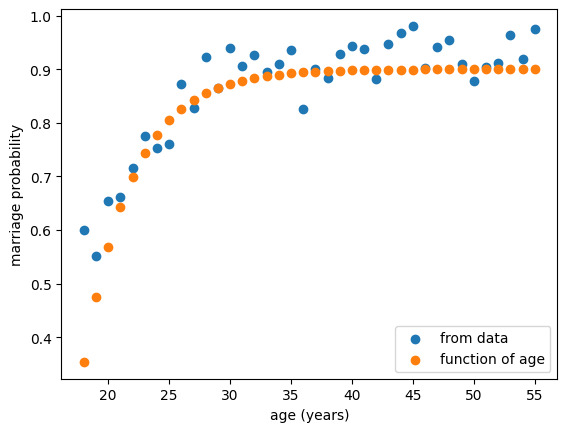
\includegraphics[width=0.4\textwidth]{img/exp_marr.jpeg}
\caption{Probability of {\tt marriage} against {\tt age}}
\label{fig:exp_marriage}
\end{figure}

If ``treat" is equal to one, we sample a treatment effect from a gaussian with mean 5000 and standard deviation 500 and add it to the re78 values of treated patients (Previously we tried to sample the ATE based on the experimental data, but because some combinations with one or two people in the experimental data had huge treatment effects, this skewed the estimate significantly and made it harder to see if the method was working correctly). In a way, we're exaggerating our ATE so it's easier to measure with our propensit-based strata method. This way, the confounders do influence treatment and the real income, but its increase upon treatment is very clear this way.

Although the real earnings in 1978 after the treatment are impacted by a number of confounders (and the likelihood of treatment depends on this as well), the average effect of setting ``treat" to one is homogeneous and equal to an increase in income of 5000USD. We use the previously explained approach of computing stratified propensities and apply it to the synthetic dataset. Figure \ref{fig:strata} shows the estimated effect as a function of the number of strata. The result is plausible and relatively close to the true value of 5000USD.

\begin{figure}[ht]
\centering
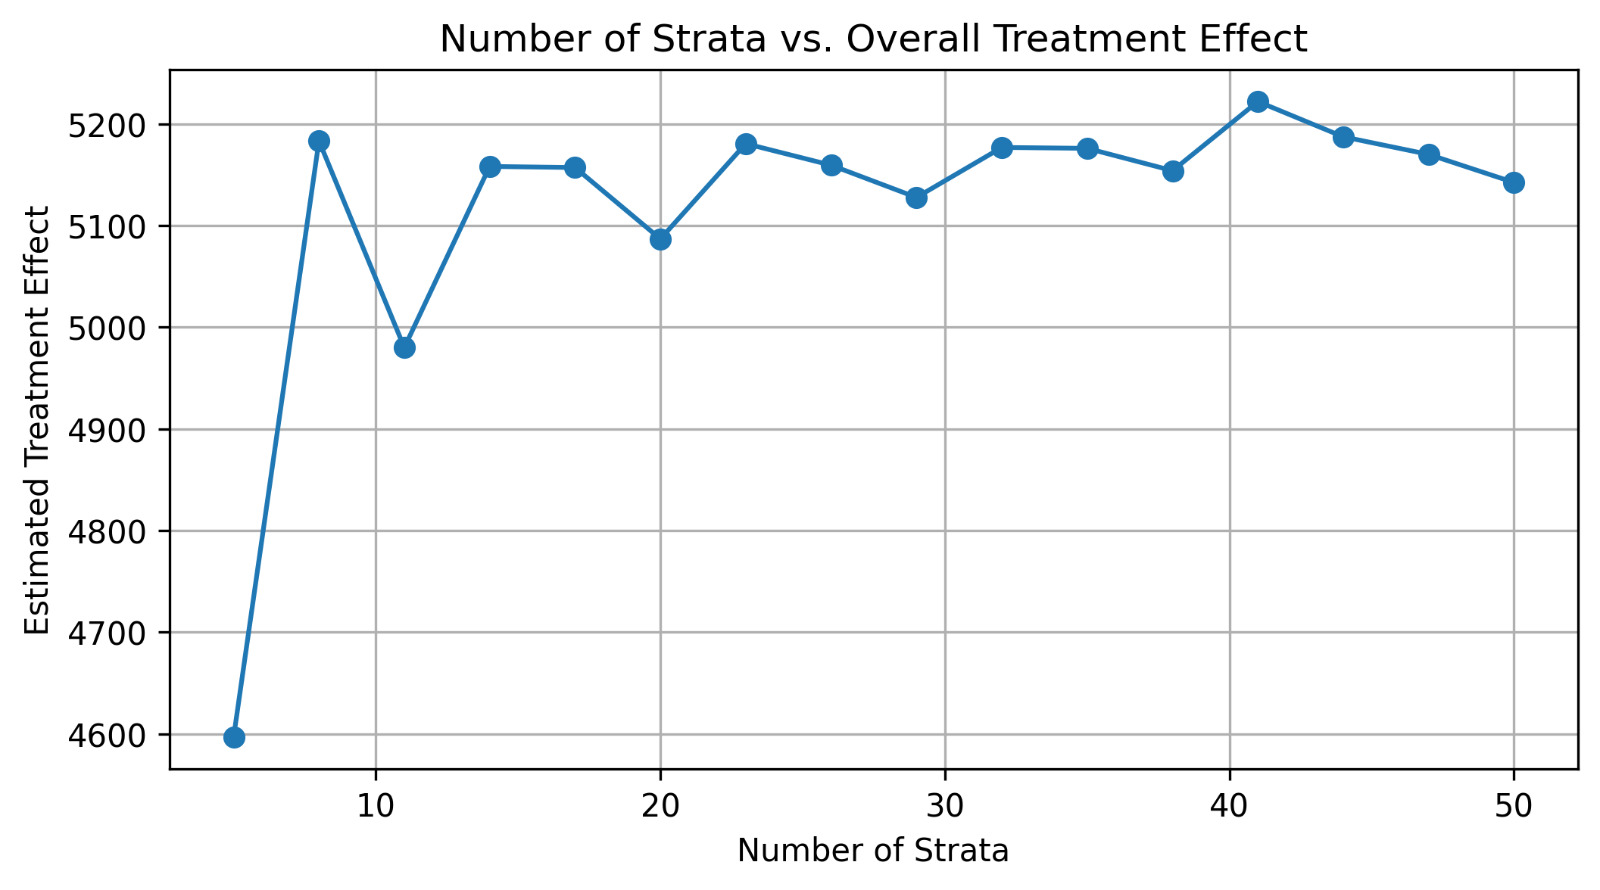
\includegraphics[width=0.6\textwidth]{img/ate_strata.jpeg}
\caption{Number of Strata vs Average Treatment Effect}
\label{fig:strata}
\end{figure}

\section{Next steps for the project} \label{sec:next_steps}

\begin{itemize}[itemsep=-0.25em]
\item{Heterogeneous treatment effects for each subgroup: This would help us understand how job training affects a certain race, education, age group or those with lower starting salaries.}
\item{Sensitivity Analysis: We want to understand how including additional covariates that represent potential unmeasured confounders impacts the propensity score. This would help assess how sensitive the results are to the inclusion of these unmeasured variables. For example, we could measure mental state or criminal history and understand its impact.}
\item{Selection Bias: We need to adjust and understand how selection bias may impact our dataset ``in the wild". Since the original study was a randomized control trial, a causal effect was readily available. However, for our observable dataset, we need to understand the impact of limiting our subset to the male only population and }
\end{itemize}

\section{Ask for feedback}

We are unsure whether our causal risk estimate for the counterfactual was calculated correctly and we require feedback. We will discuss this over our weekly call. We also would like to understannd how HTEs are calculated through our upcoming classes.


\bibliographystyle{plain}
\bibliography{references}


\clearpage


\end{document}
